\subsection{Algoritmos de Ordenamiento}

Al probar los algoritmos de ordenamiento, se ven grandes diferencias en la práctica, a pesar de que en teoría todos operan en $O(n \log n)$. Para los algoritmos podemos comentar que para;

\textbf{1. Merge Sort:} 
Para casi todas las pruebas, Merge Sort terminó siendo el más lento (tardando más de 1200 ms con $10^7$ datos aleatorios). El problema no son las comparaciones,
sino que es un algoritmo del tipo \textit{out-of-place}, es decir, requiere memoria adicional proporcional al tamaño del arreglo original O(n) para poder realizar el sort.
Al estar creando vectores temporales (\texttt{std::vector}) y copiando datos a cada rato, el procesador se satura manejando la memoria.

\textbf{2. Quick Sort:}
Durante las primeras pruebas, la implementación clásica de Quick Sort \cite{gfg_quick_sort} colapsó, como teniamos que elegir siempre el último elemento como pivote y usar partición simple,
el algoritmo caía en su peor caso ($O(n^2)$) frente a arreglos ya ordenados o con muchos datos repetidos (Dominio D1), tardando una eternidad.
Tras solucionar esto cambiando el pivote al centro e implementando la partición de 3 vías (llamado \textit{Dutch National Flag} en internet \cite{gfg_3way_quicksort}),
Quick Sort y std::sort no tuvieron más problemas y funcionaron excelente. Como son algoritmos \textit{in-place} y solo hacen intercambios (\texttt{swap}) en la misma memoria,
aprovechan súper bien la memoria caché. Llamó mucho la atención lo rápido que fue \textsc{Quick Sort} en el Dominio D1, lo que confirma que el \textit{Dutch National Flag}
fue un éxito total, ya que agrupa los repetidos, los ignora para la siguiente recursión y achica bastante el árbol recursivo.

\textbf{3. Patience Sort:}
Después de optimizarlo con búsqueda binaria (\texttt{std::lower\_bound}) y usando un Min-Heap para la cola de prioridad, el Patience Sort logró un crecimiento súper estable.
Si bien es un poco más lento que los algoritmos \textit{in-place} por todo el trabajo de mantener el stack y el heap,
demostró ser una opción muy robusta para procesar millones de datos sin ningún problema.

\textbf{4. Análisis general y de memoria:}
Al analizar las curvas, se observa un disparo abrupto en los tiempos a partir de $N=10^5$. Este comportamiento obedece a dos factores críticos.
En primer lugar, la escala de las gráficas condensa la inyección de 9.900.000 datos exclusivamente en el último tramo,
haciendo que el salto asintótico se vea visualmente desproporcionado.
En segundo lugar, existe un limite fisico del hardware,
un arreglo de $10^5$ enteros (aproximadamente 400 KB) cabe holgadamente en la memoria rapida del procesador (como los 12 MB de caché L3 que tiene el Intel Core i5-10400F donde se ejecutaron las pruebas).
Operar aquí garantiza latencias mínimas. Sin embargo, al procesar $10^7$ elementos, la estructura pasa a pesar 40 MB, rebasando por completo la capacidad de la caché y
obligando a la CPU a buscar datos en la RAM. Esto explica por qué el rendimiento de \textsc{Merge Sort}
se degrada tan severamente en el último tramo: al ser out-of-place, crea vectores
temporales que duplican la memoria a casi 80 MB, saturando el bus de datos hacia la RAM mucho más rápido que las alternativas in-place.

\begin{figure}[H]
    \centering
    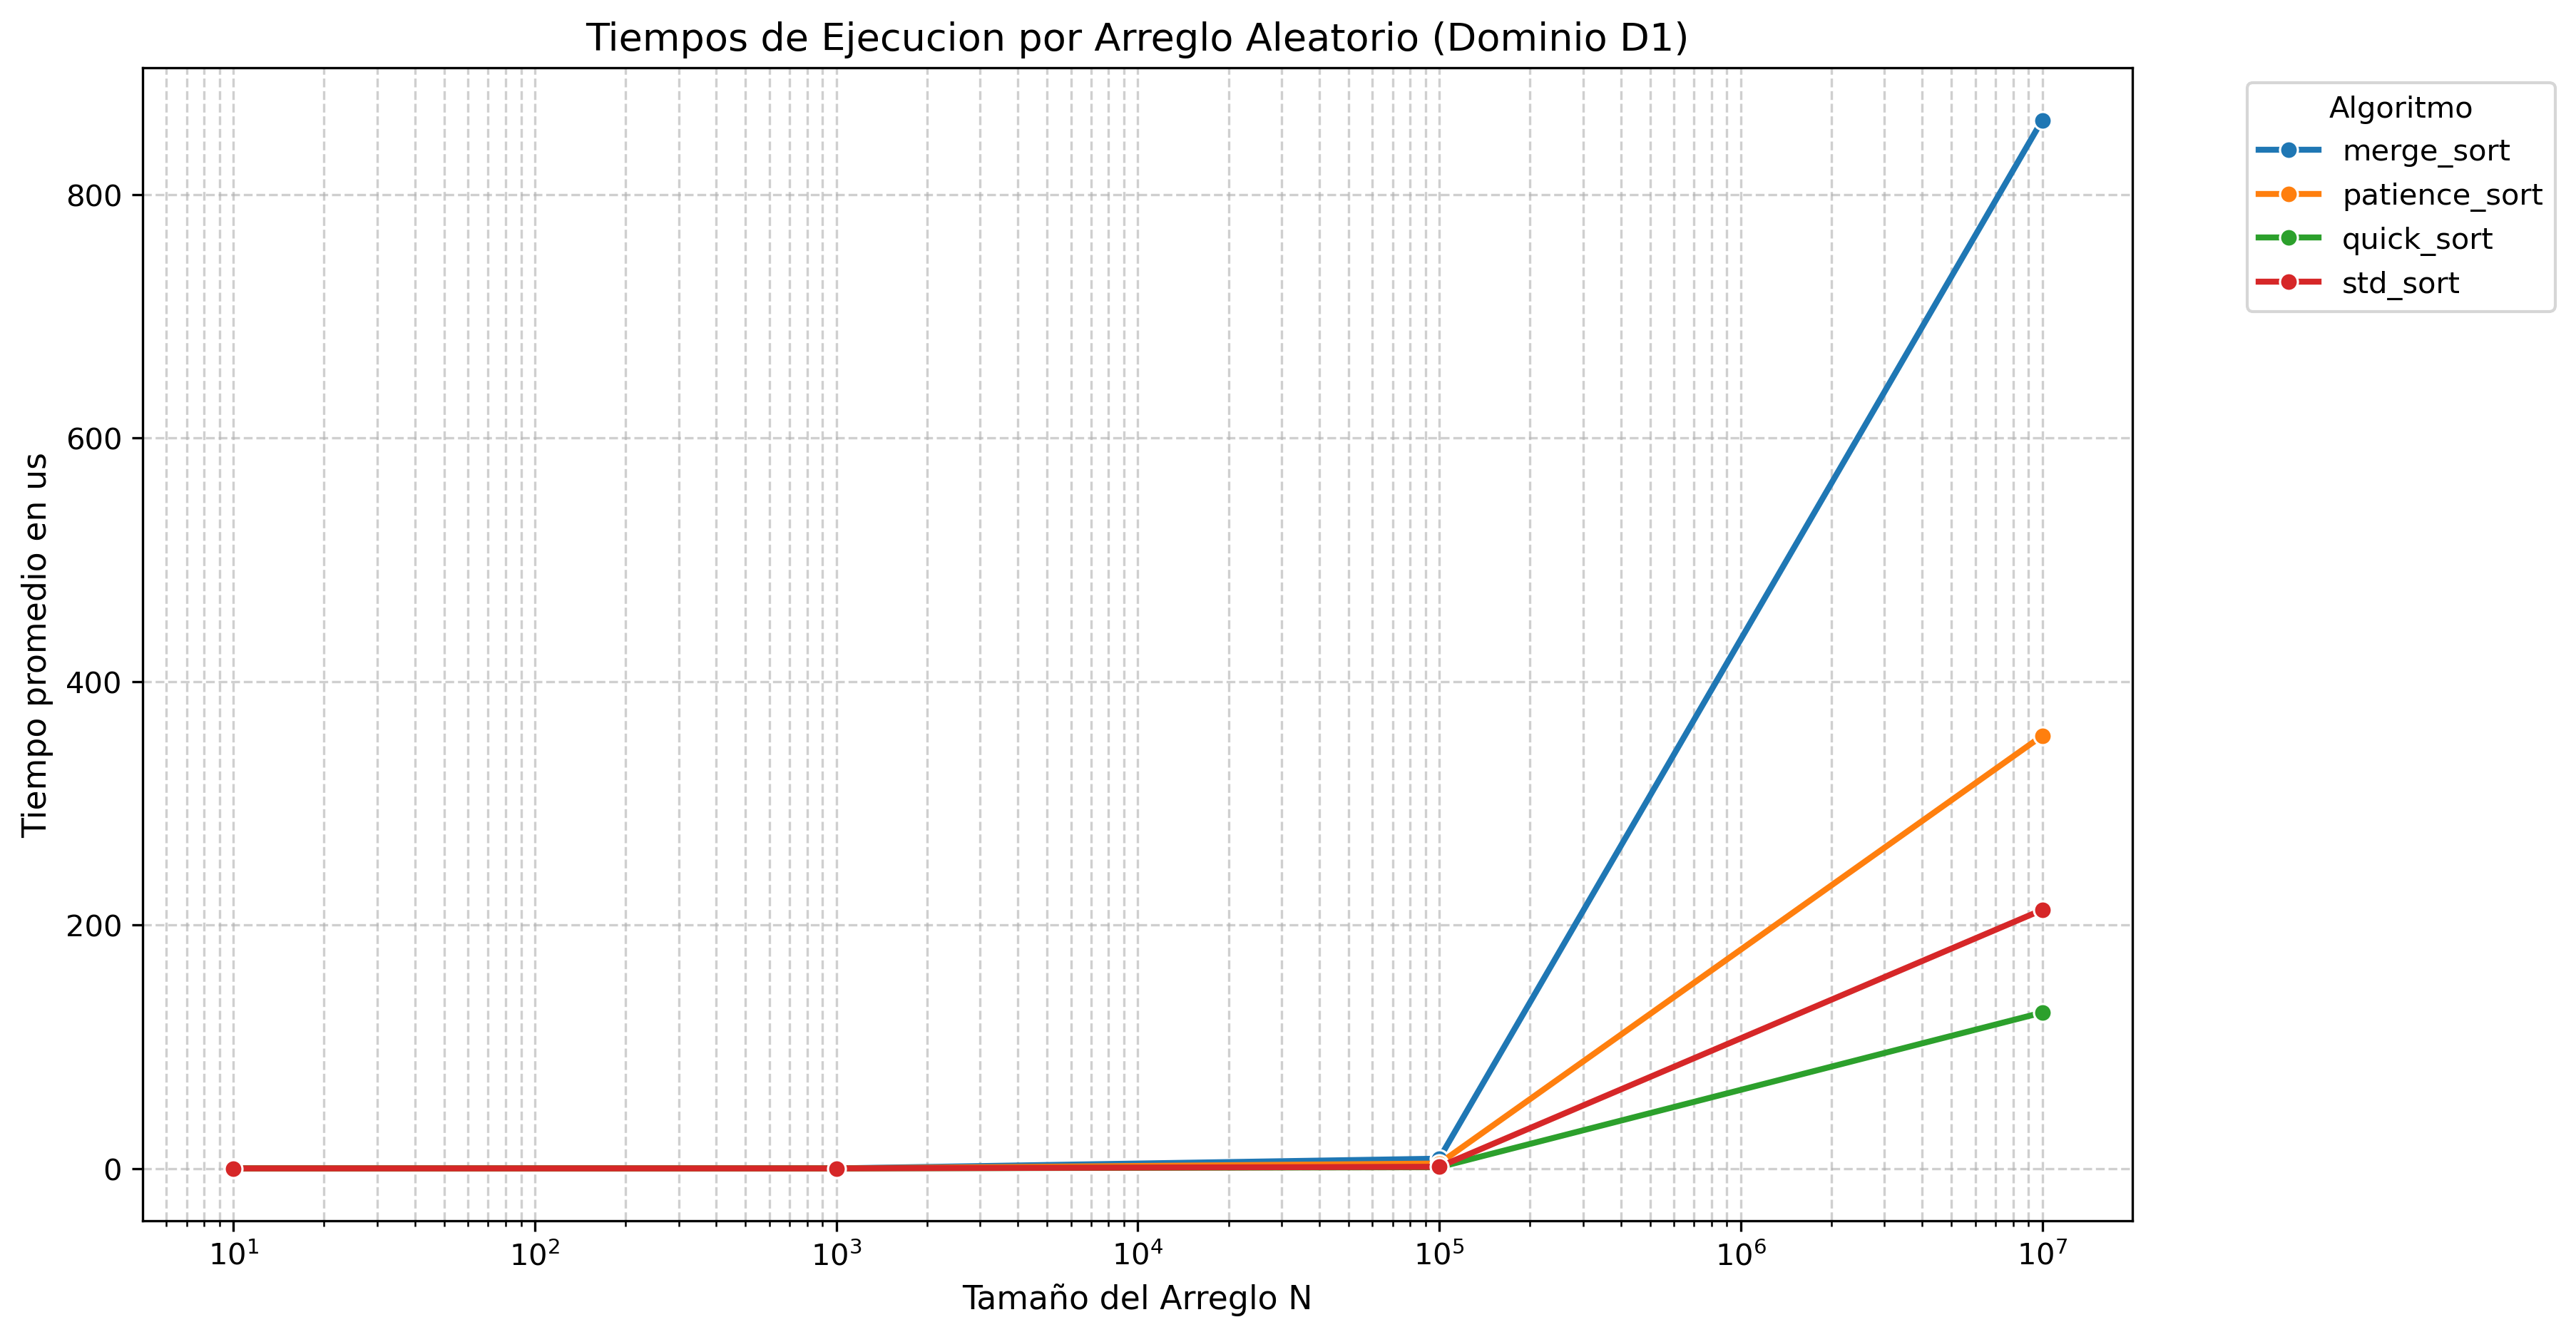
\includegraphics[width=0.85\textwidth]{../code/sorting/data/plots/plot_aleatorio_D1.png}
    \caption{Arreglo Aleatorio (D1)}
    
    \vspace{0.8cm}
    
    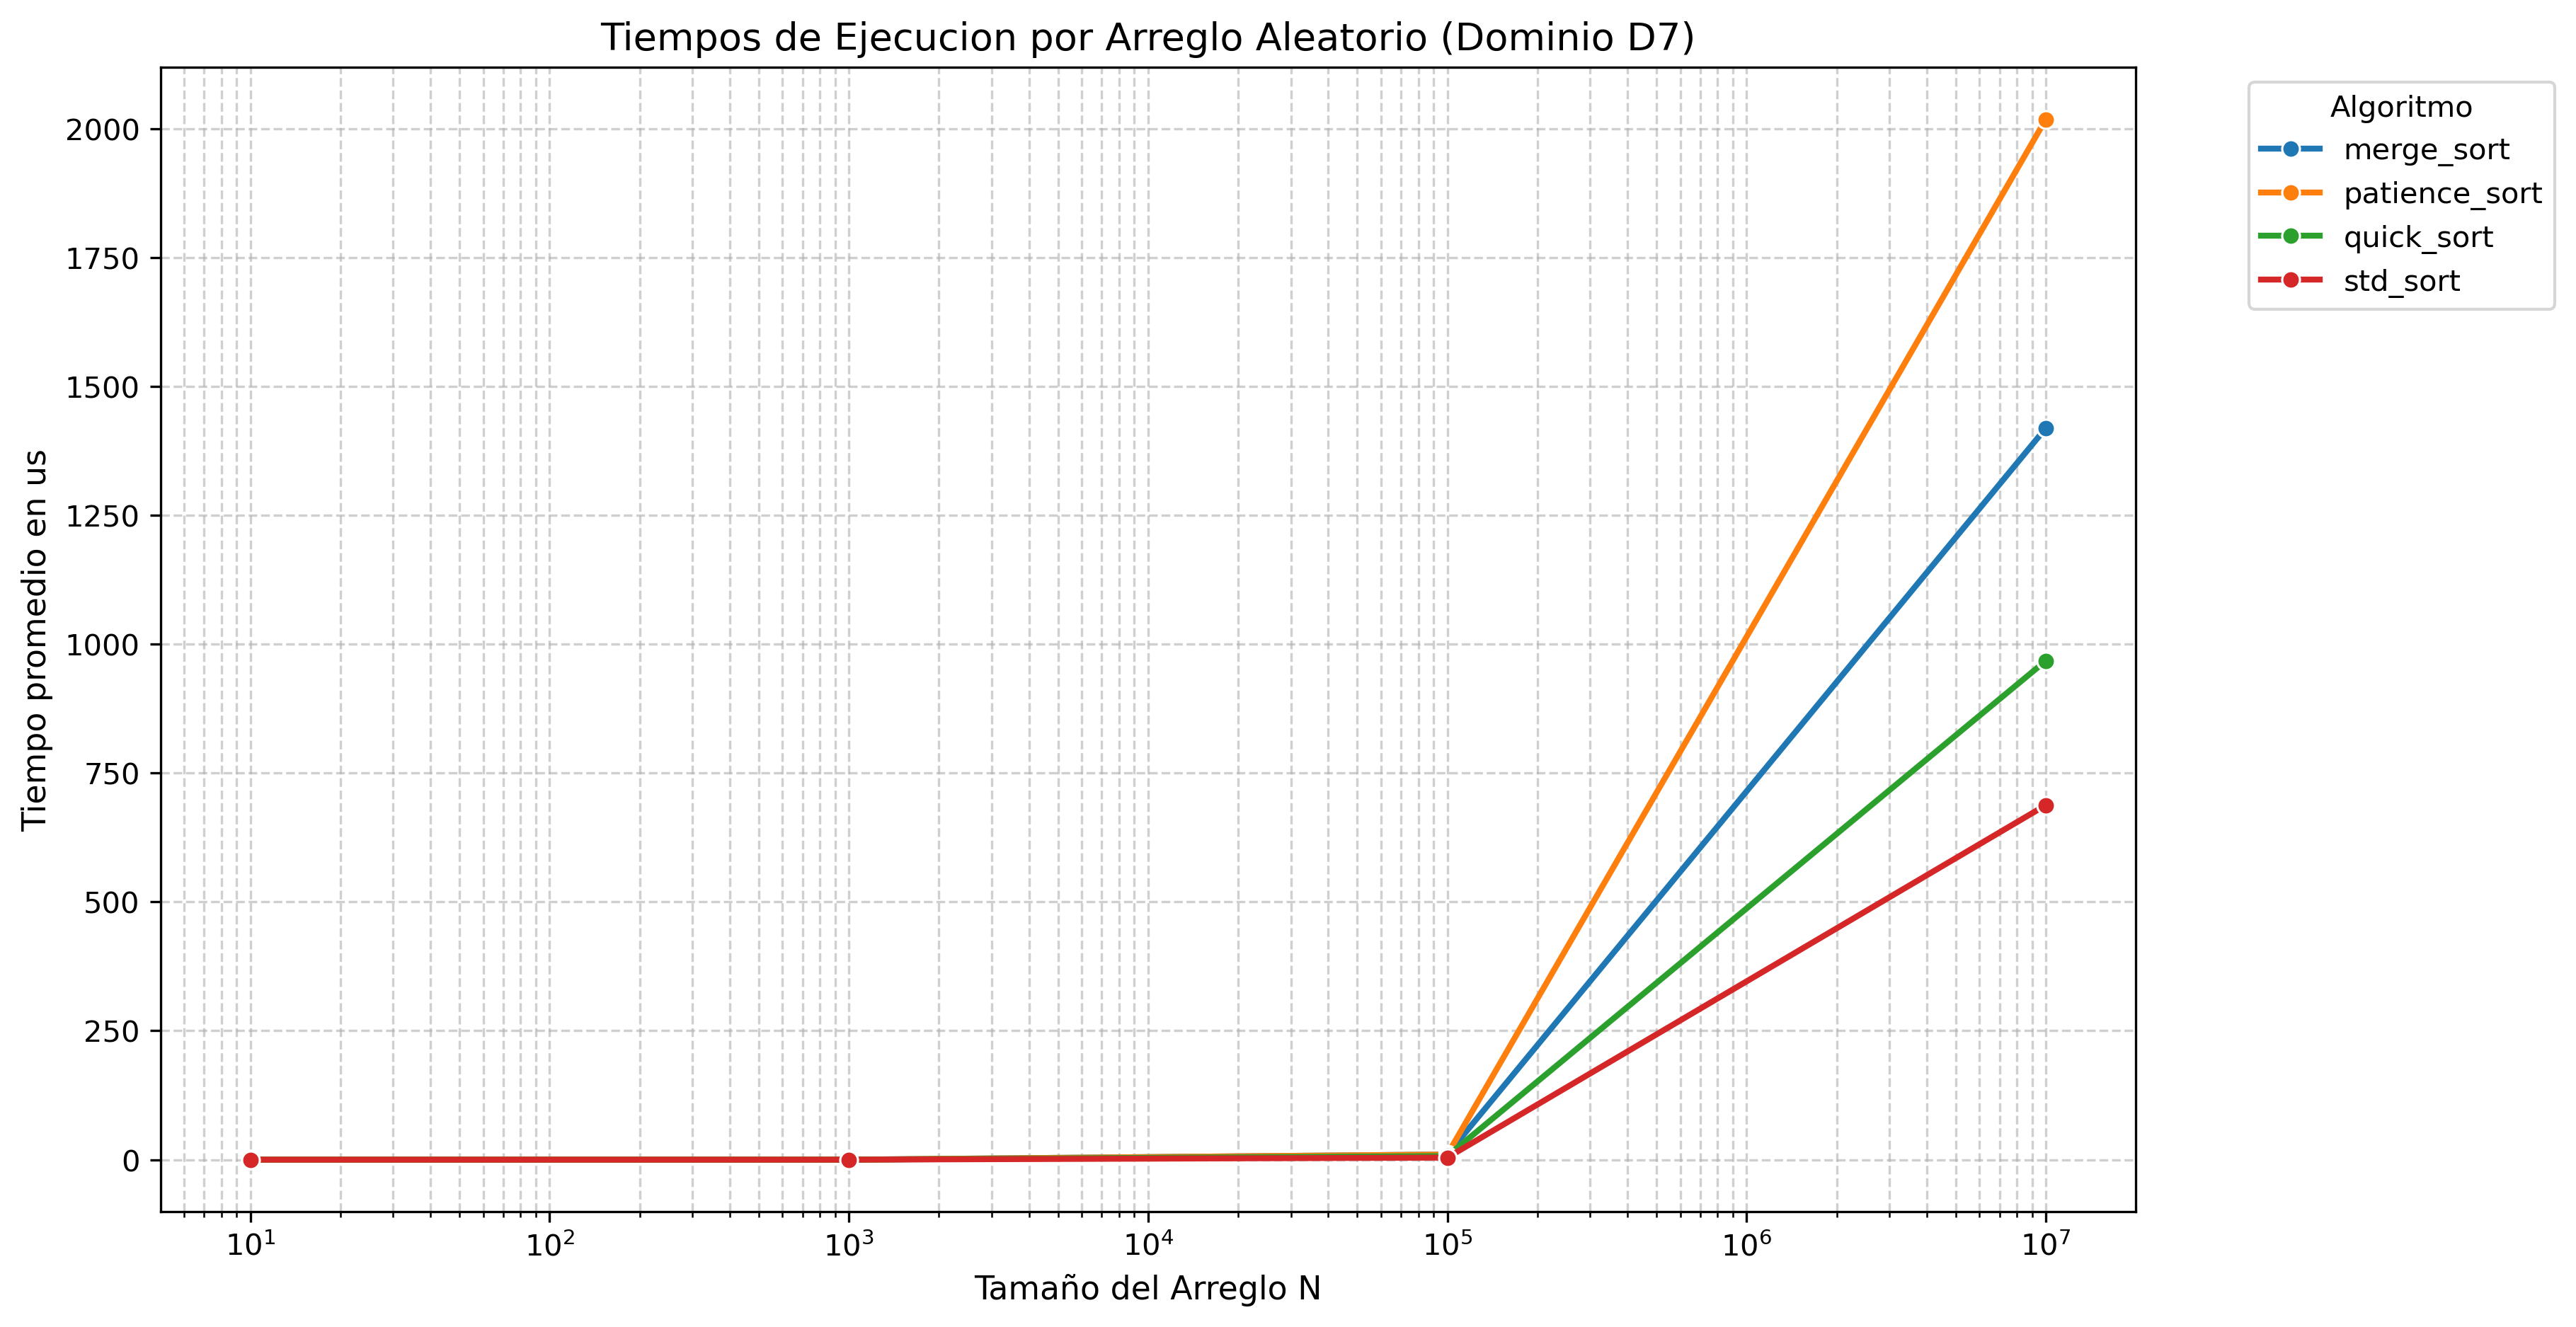
\includegraphics[width=0.85\textwidth]{../code/sorting/data/plots/plot_aleatorio_D7.png}
    \caption{Arreglo Aleatorio (D7)}
\end{figure}

\begin{figure}[H]
    \centering
    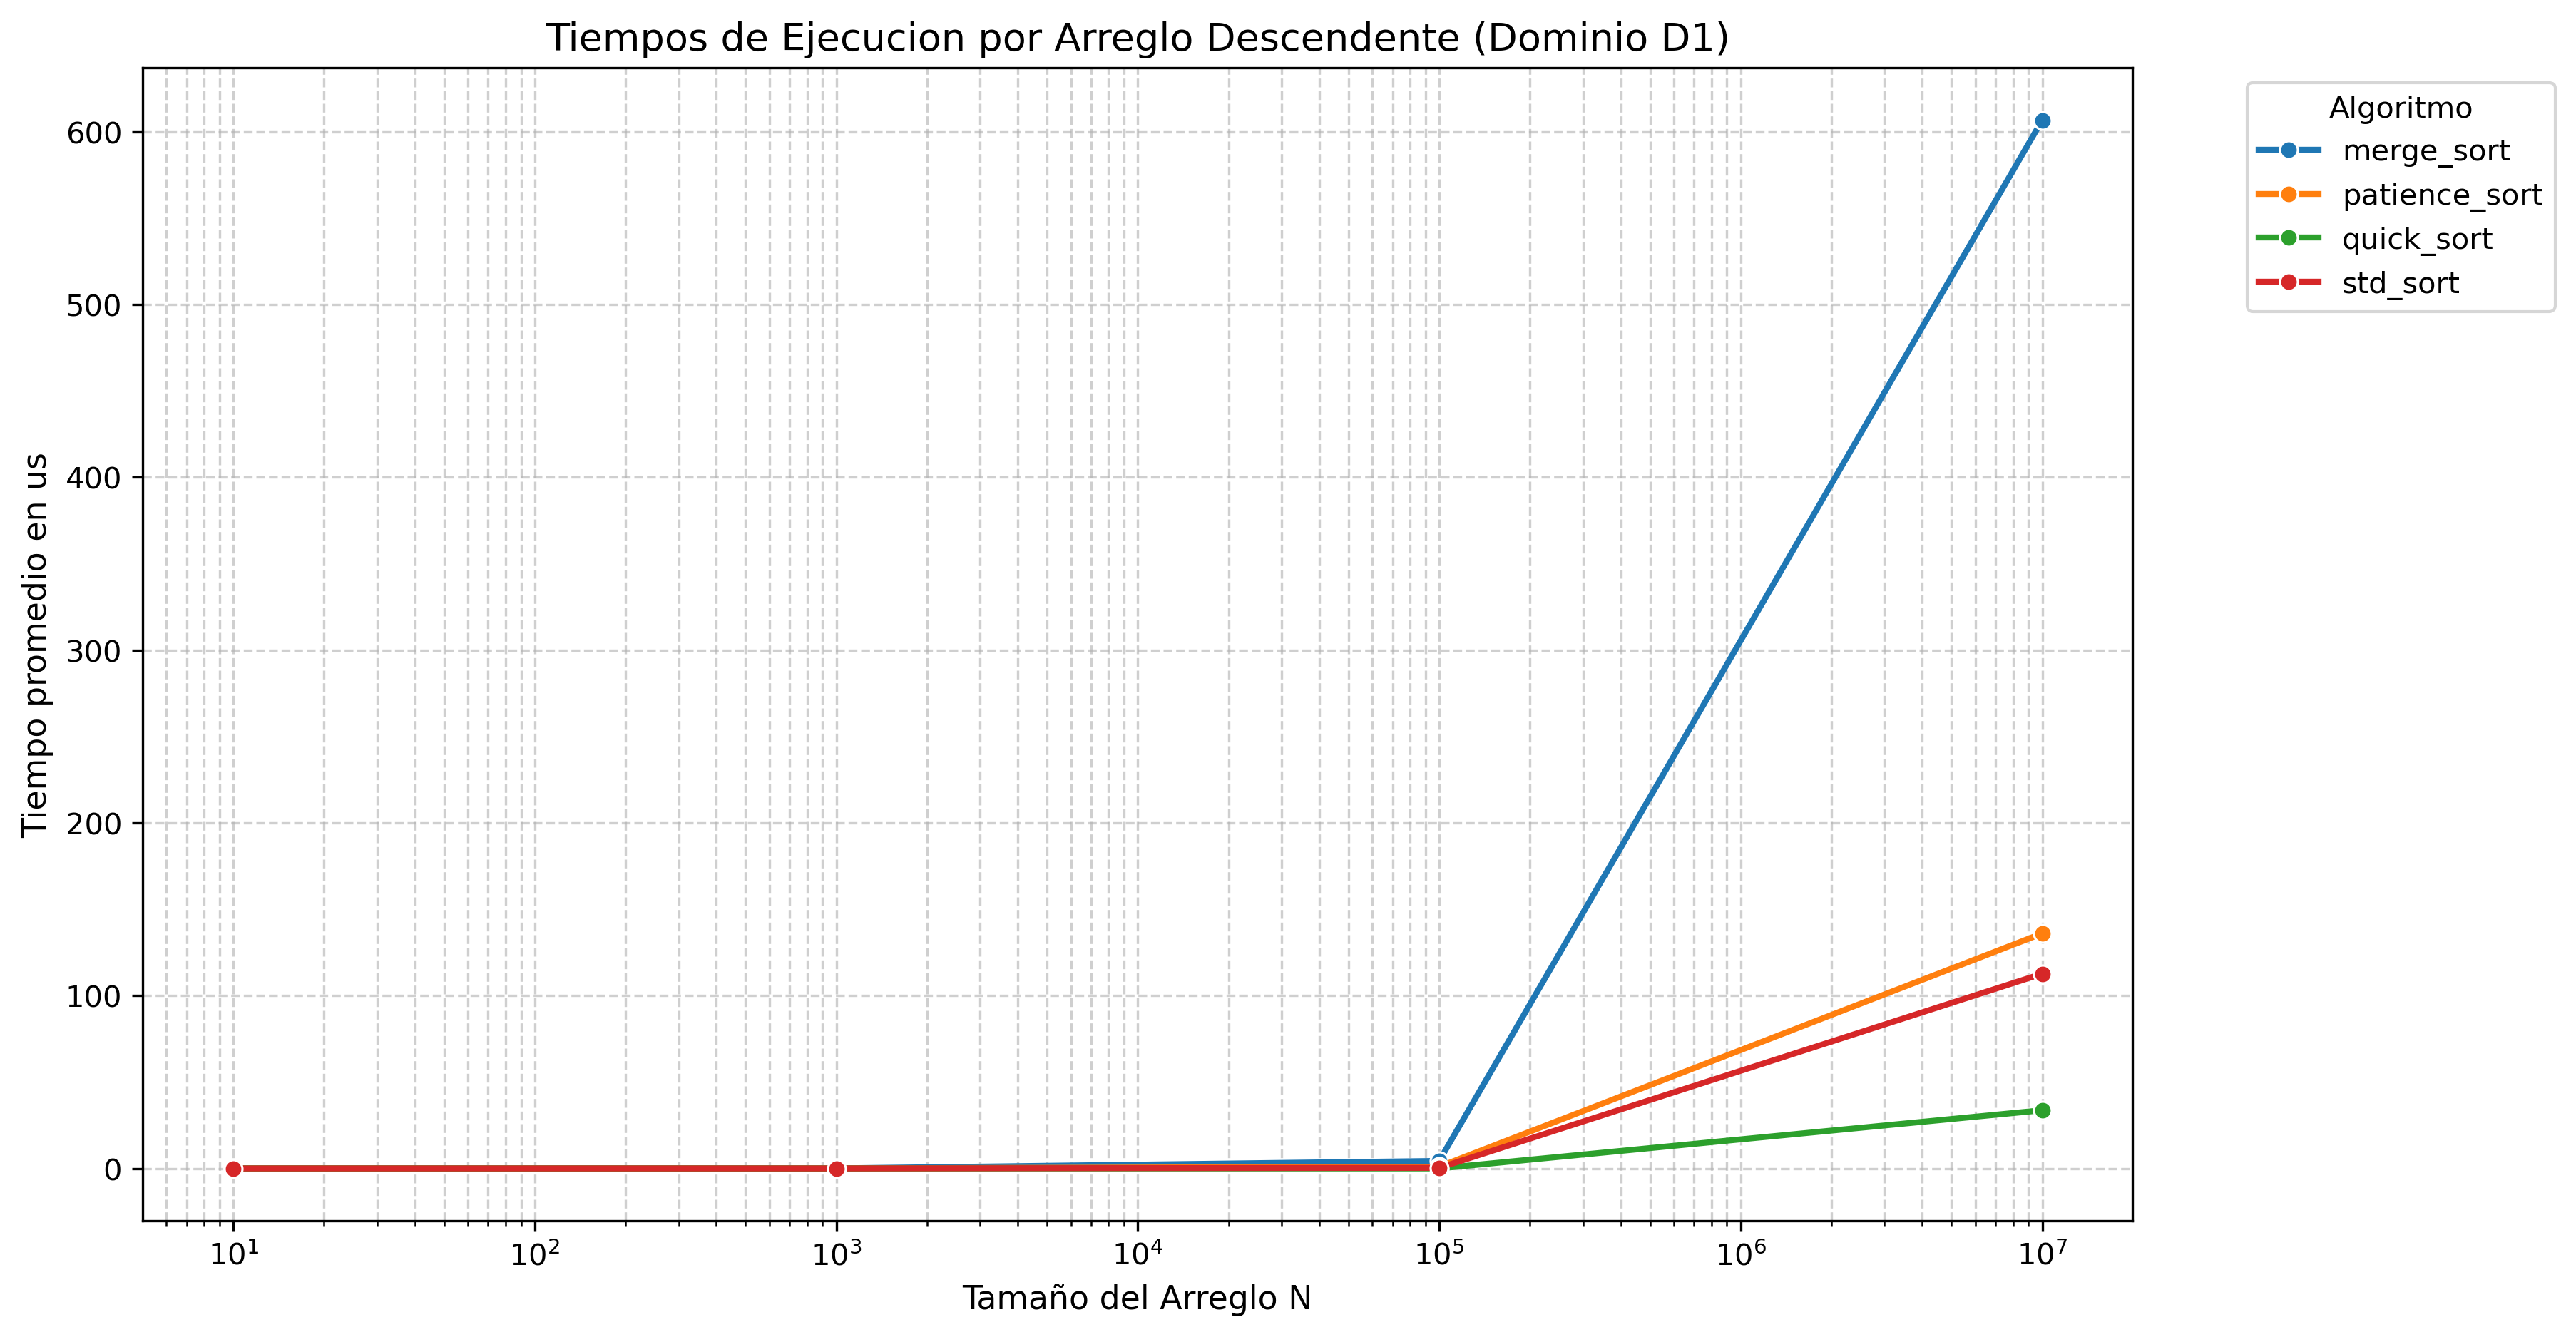
\includegraphics[width=0.85\textwidth]{../code/sorting/data/plots/plot_descendente_D1.png}
    \caption{Arreglo Descendente (D1)}
    
    \vspace{0.8cm}
    
    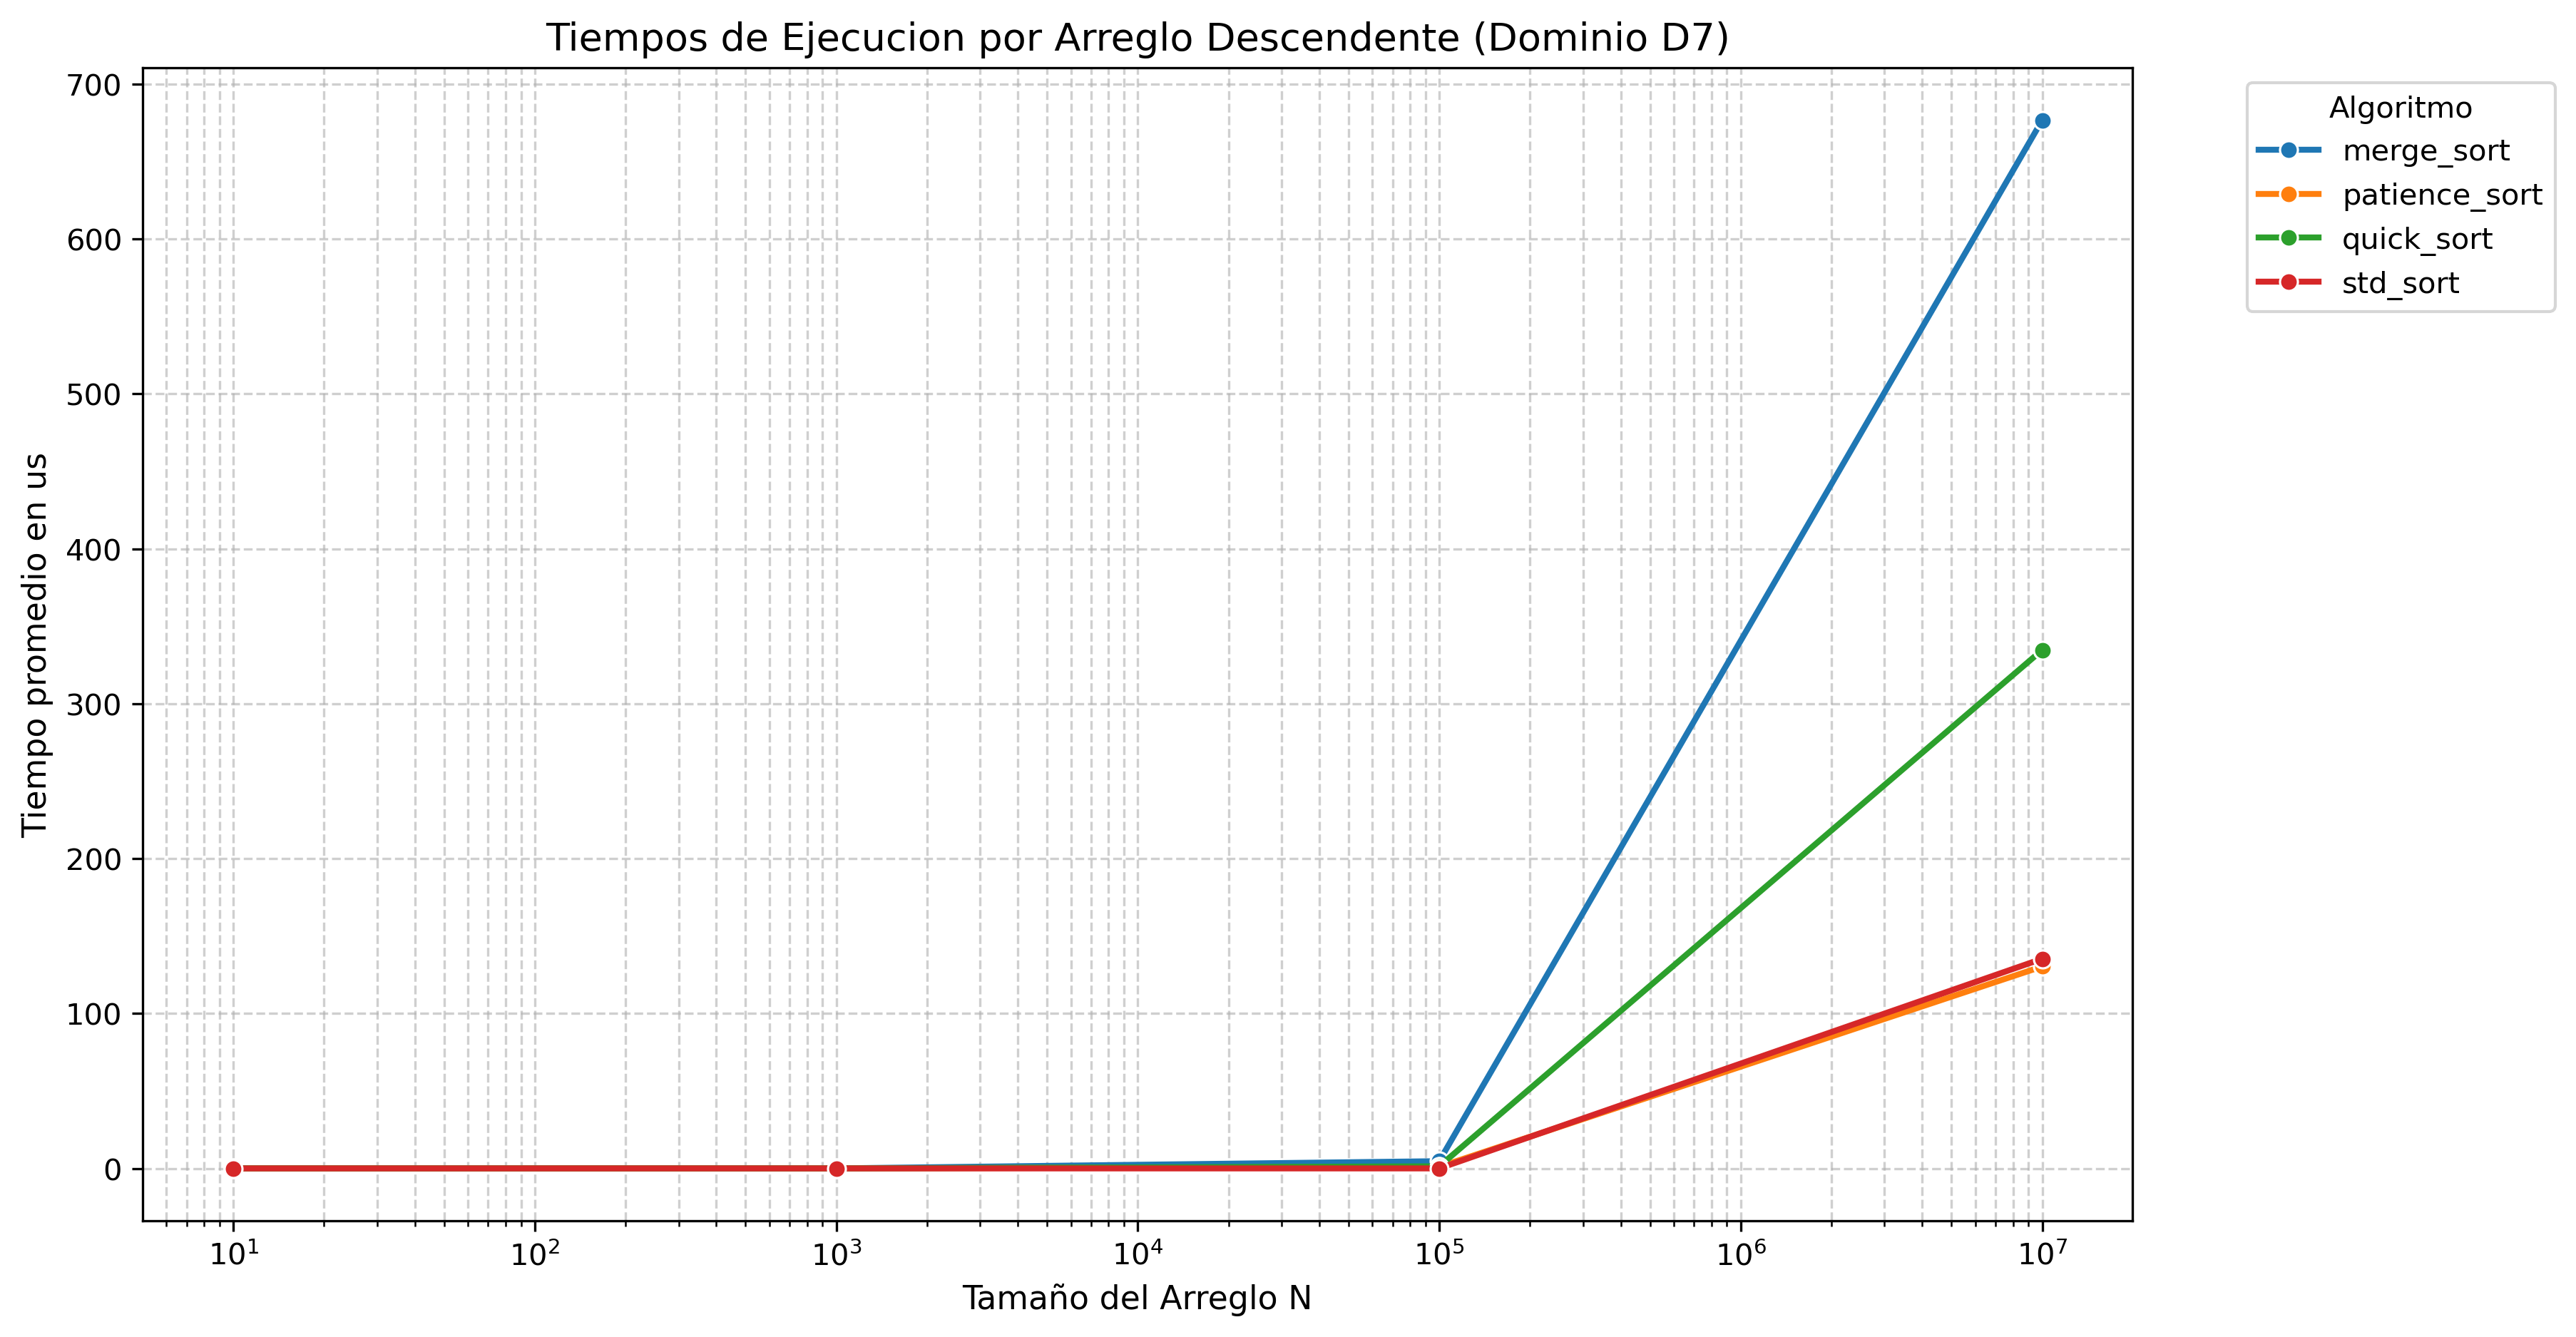
\includegraphics[width=0.85\textwidth]{../code/sorting/data/plots/plot_descendente_D7.png}
    \caption{Arreglo Descendente (D7)}
\end{figure}

Se omitieron las gráficas del arreglo Ascendente ya que su comportamiento asintótico no presenta conclusiones adicionales de interés respecto a los casos presentados.

\subsection{Multiplicación de Matrices}

Pasando a la multiplicación de matrices, encontramos con dos cosas muy interesantes en la práctica que van un poco en contra de lo que esperábamos en teoría.

\textbf{1. No importan los 0s:}
Los tiempos fueron prácticamente idénticos sin importar si la matriz era densa, dispersa o diagonal.
Esto pasa porque usamos std::vector, que no están optimizados para comprimir o ignorar los ceros,
así que nuestro programa igual multiplica todo coordenada por coordenada haciendo el mismo esfuerzo.

\textbf{2. Naive le gana a Strassen:}
Aquí vimos que el algoritmo Naive ($O(n^3)$) le ganó con creces a Strassen ($O(n^{2.81})$, demostración del valor en la cita adyacente) \cite{medium_strassen} en todos los tamaños probados (incluso hasta $N=1024$). 
Aunque la teoría dice que Strassen es mejor \cite{medium_naive}, en la práctica sufre mucho creando submatrices y pidiendo memoria nueva en cada paso recursivo. 
Naive, al tener tres simples ciclos \texttt{for}, aprovecha mucho mejor la memoria caché y termina siendo bastante más rápido para estos tamaños.

\begin{figure}[H]
    \centering
    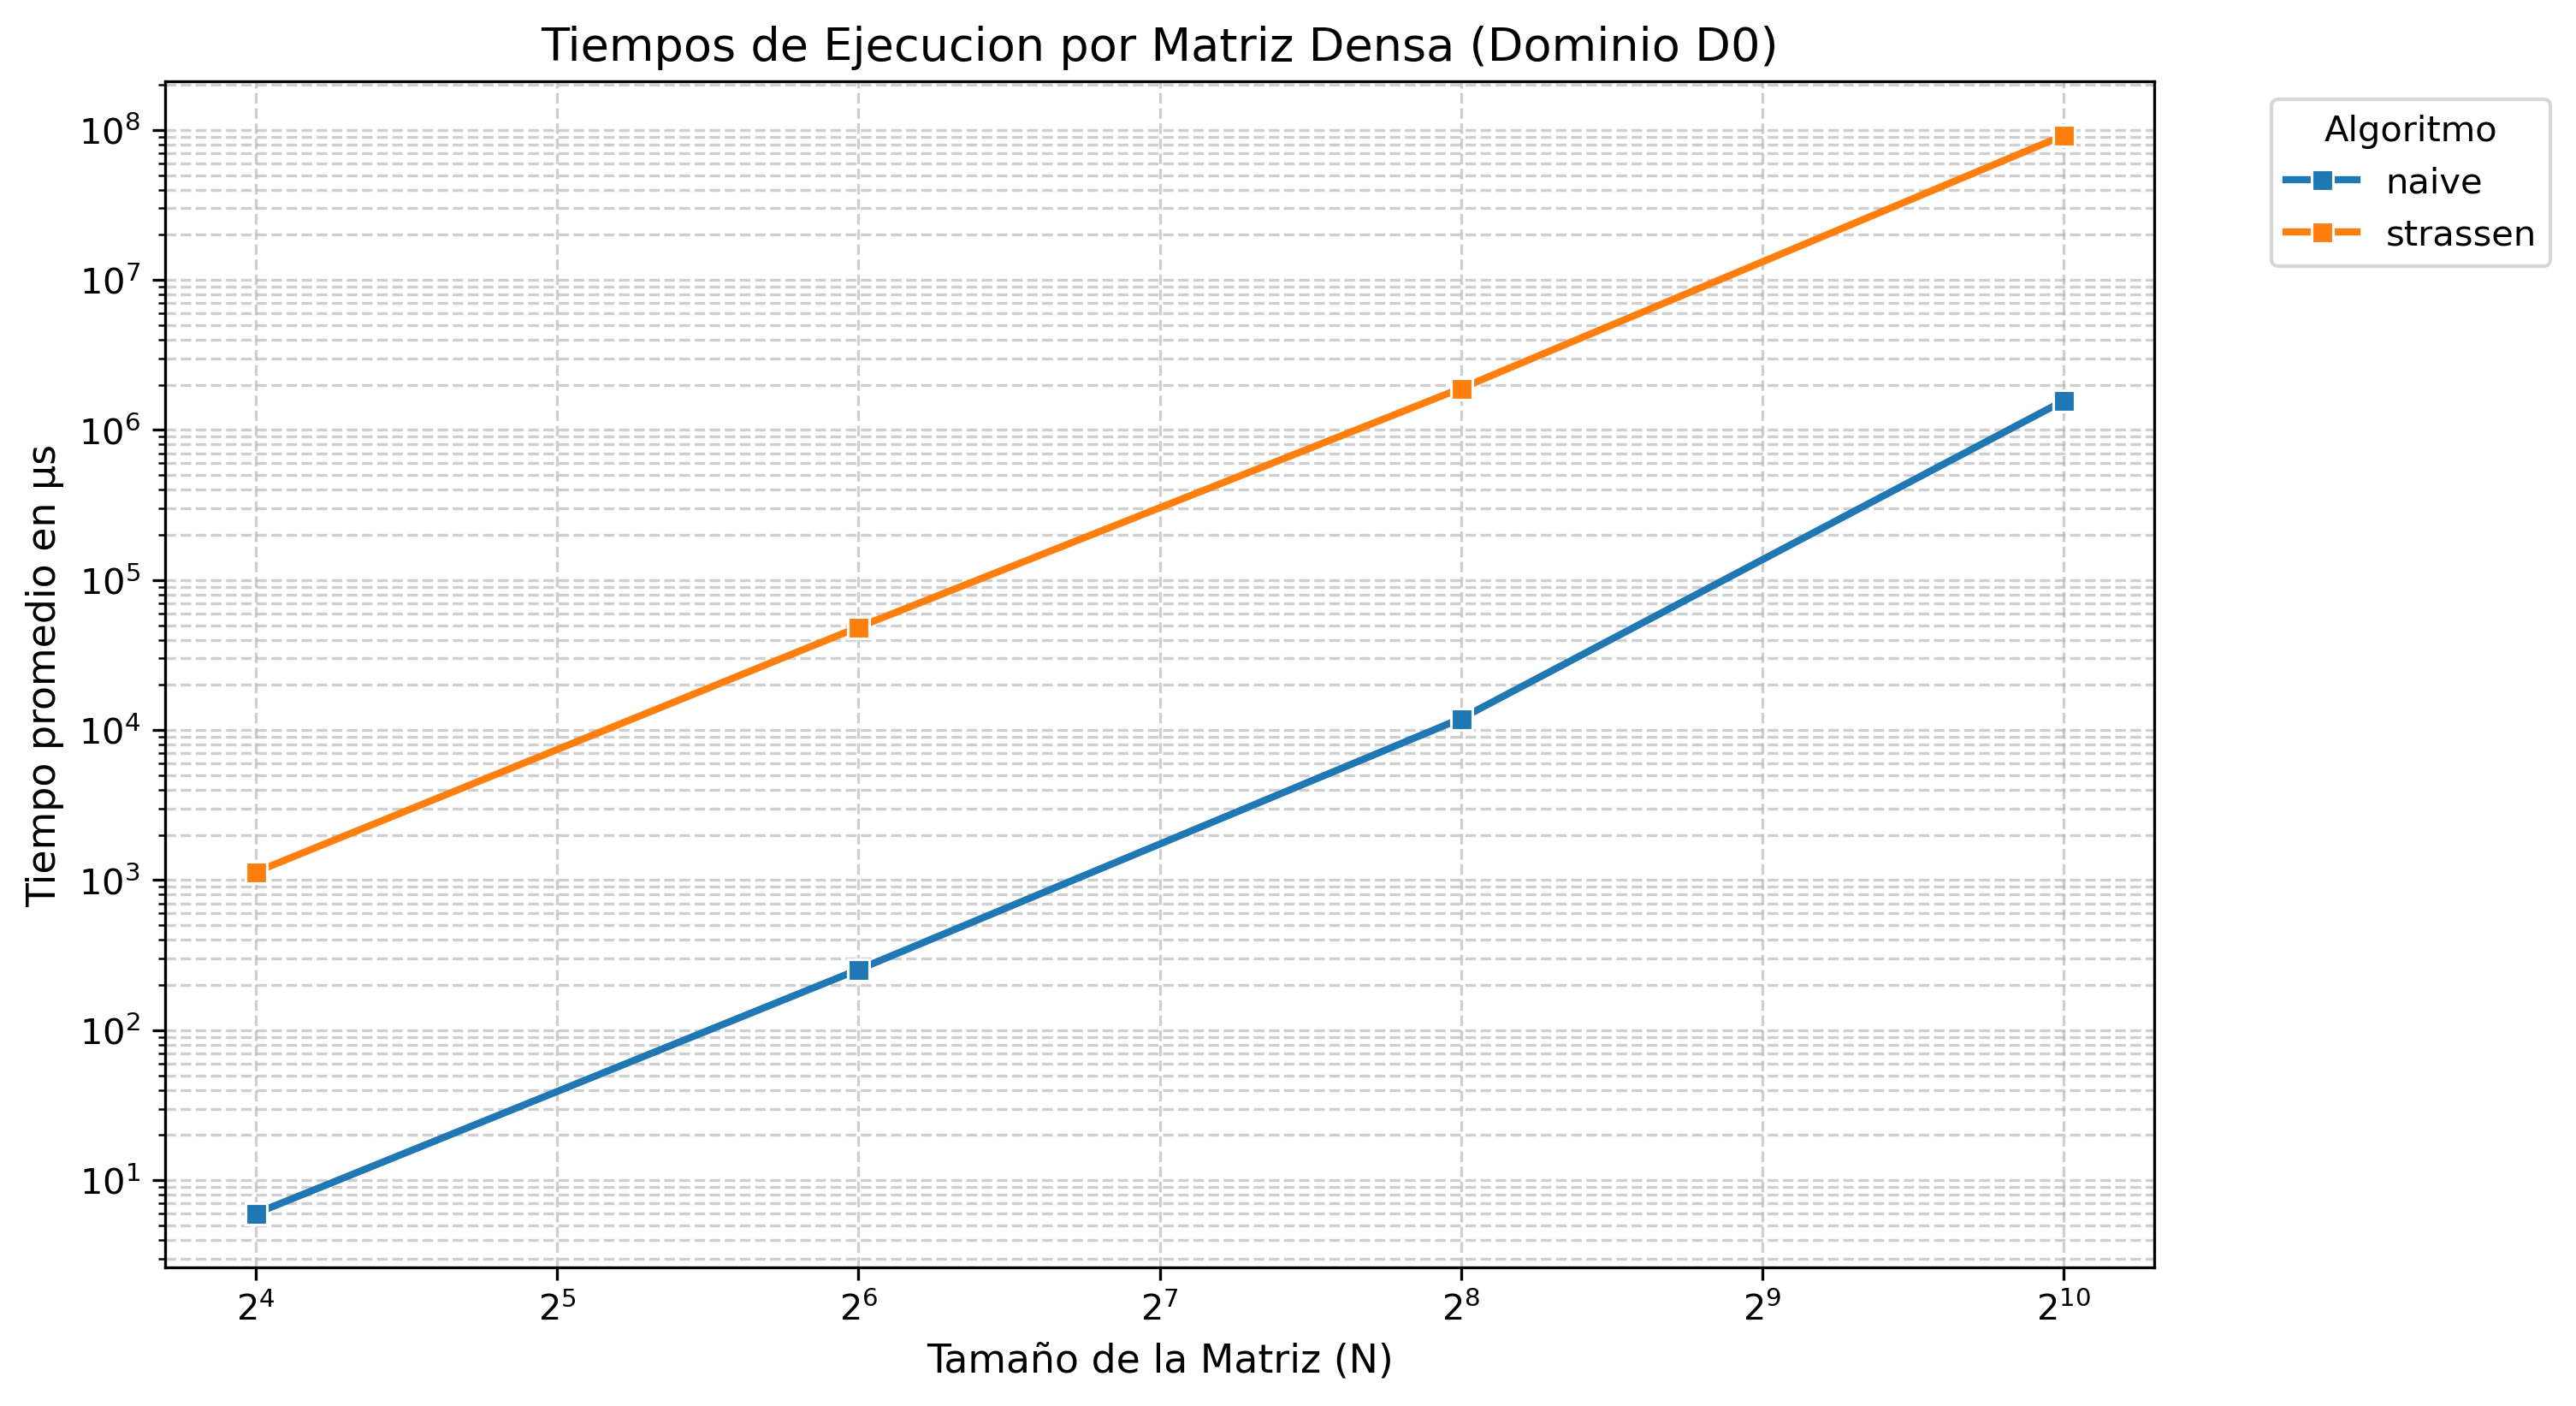
\includegraphics[width=0.85\textwidth]{../code/matrix_multiplication/data/plots/plot_densa_D0.png}
    \caption{Matriz Densa (D0)}
    
    \vspace{0.8cm}
    
    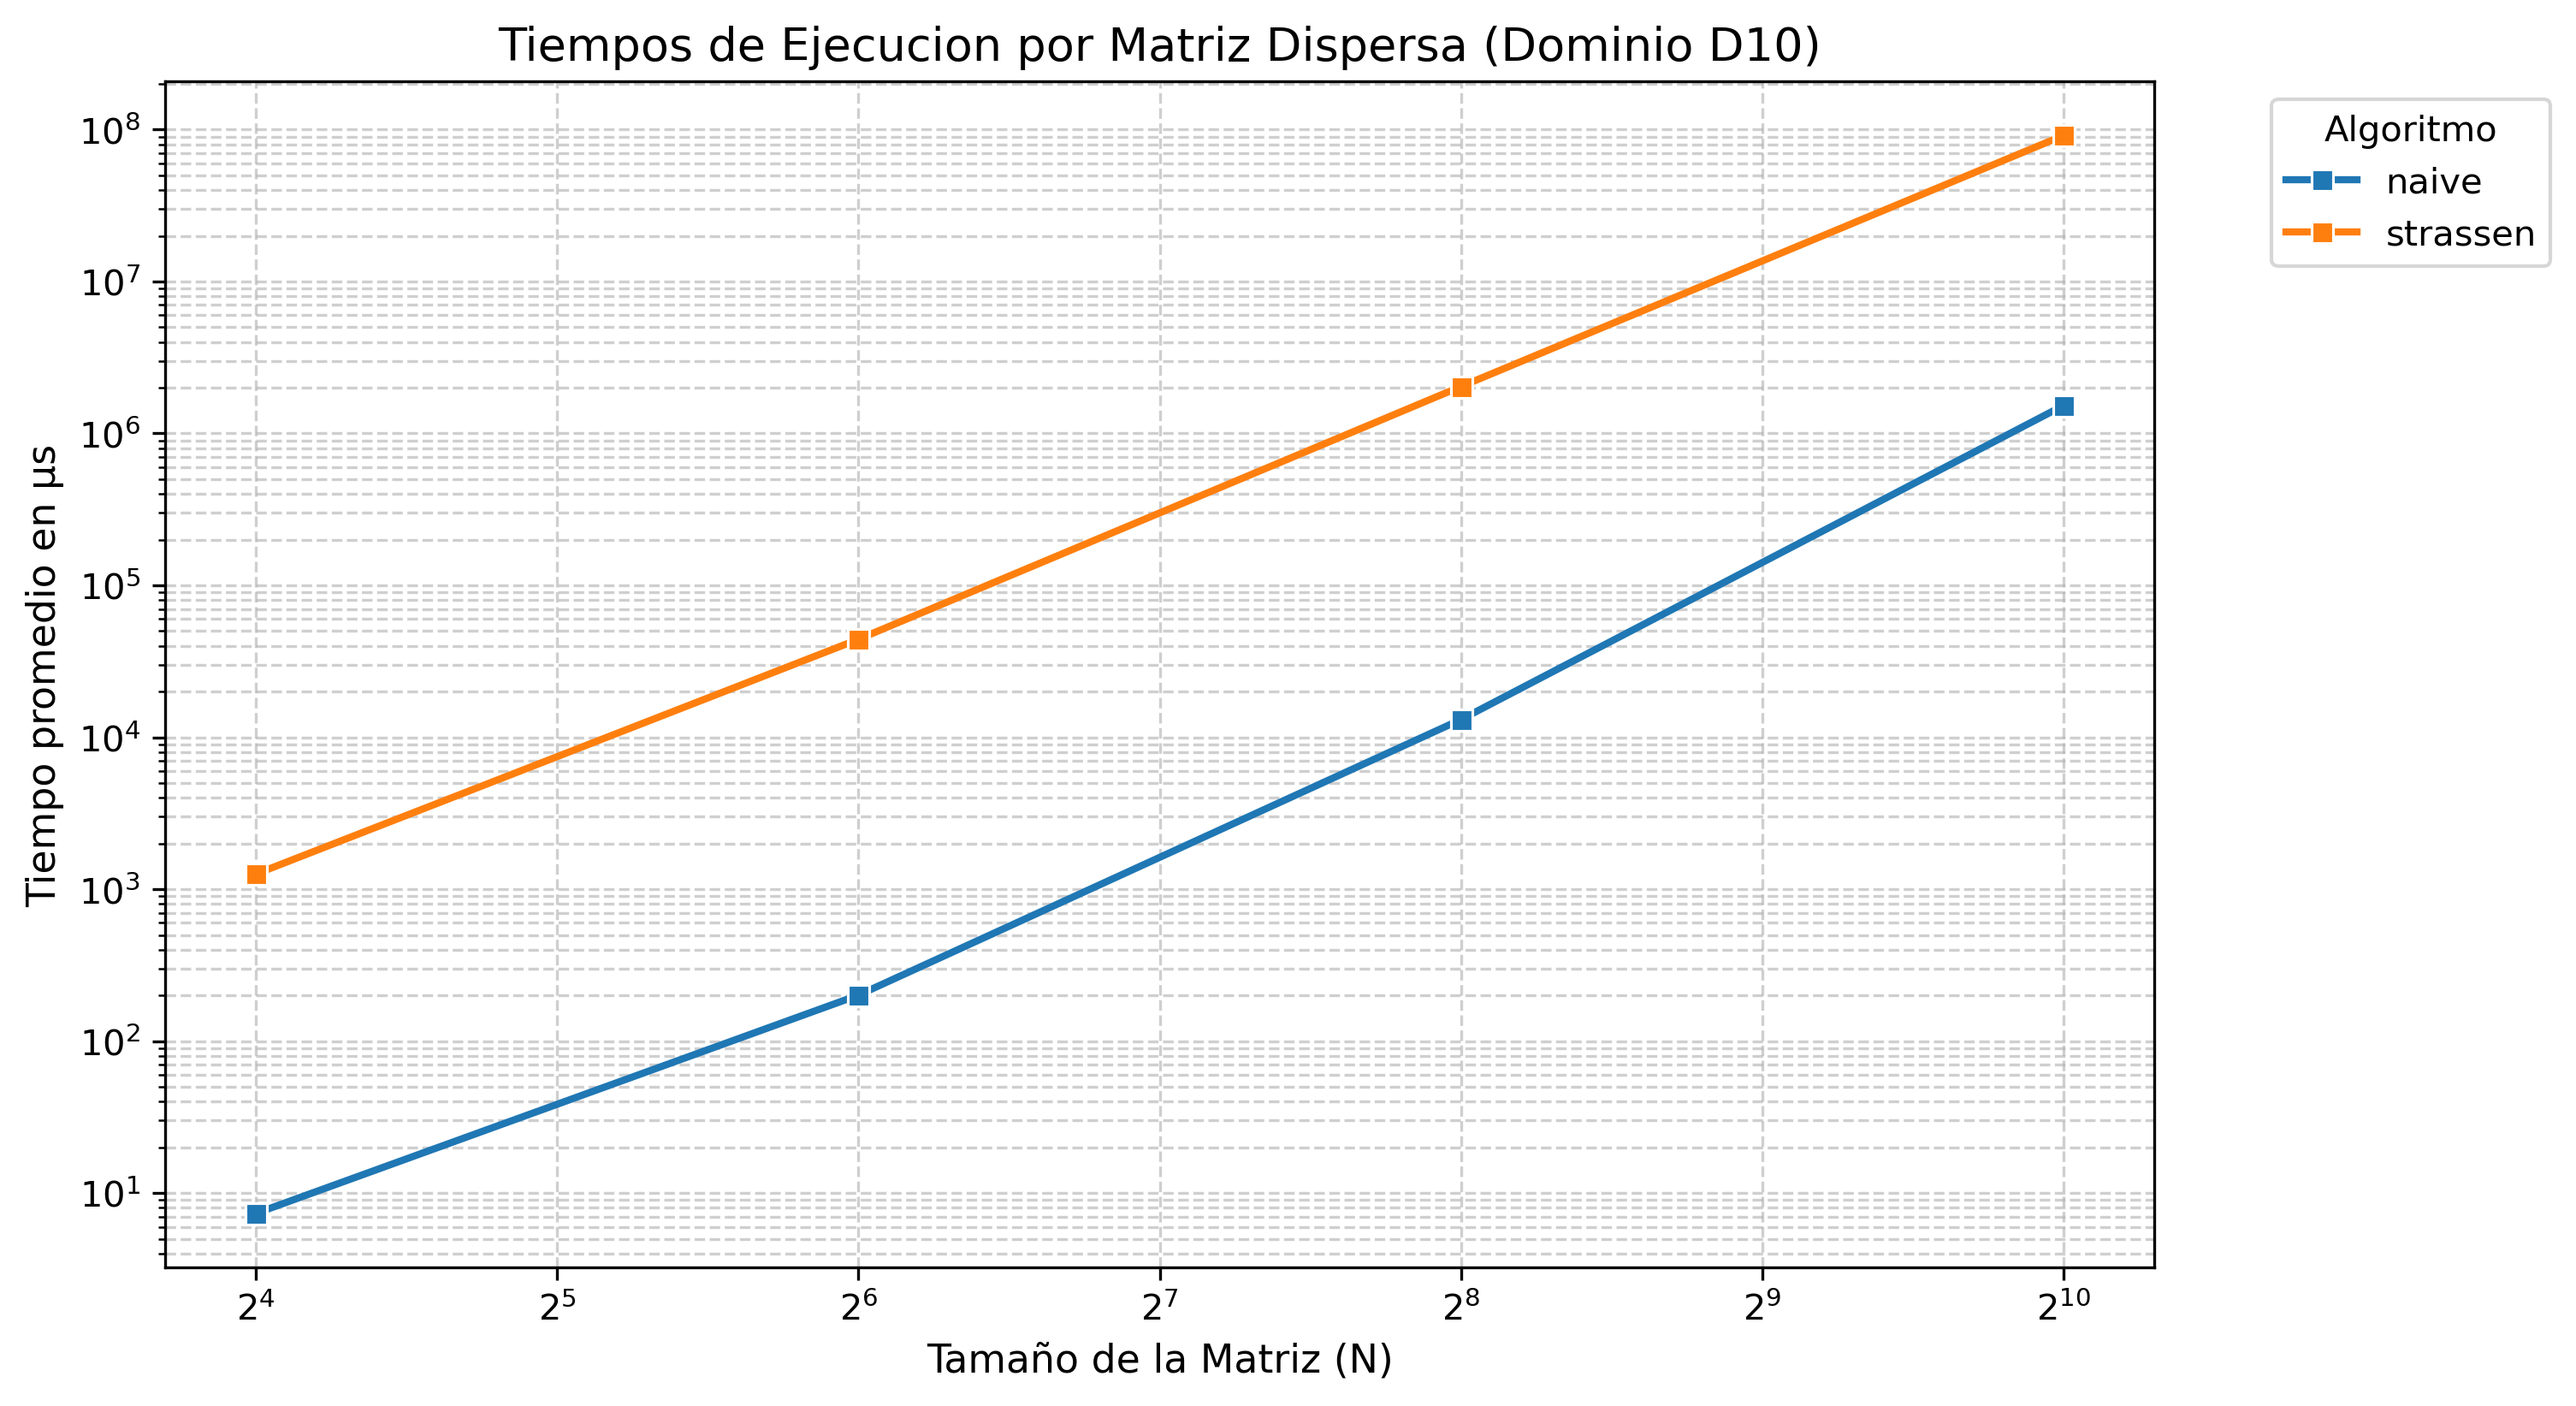
\includegraphics[width=0.85\textwidth]{../code/matrix_multiplication/data/plots/plot_dispersa_D10.png}
    \caption{Matriz Dispersa (D10)}
\end{figure}

\begin{figure}[H]
    \centering
    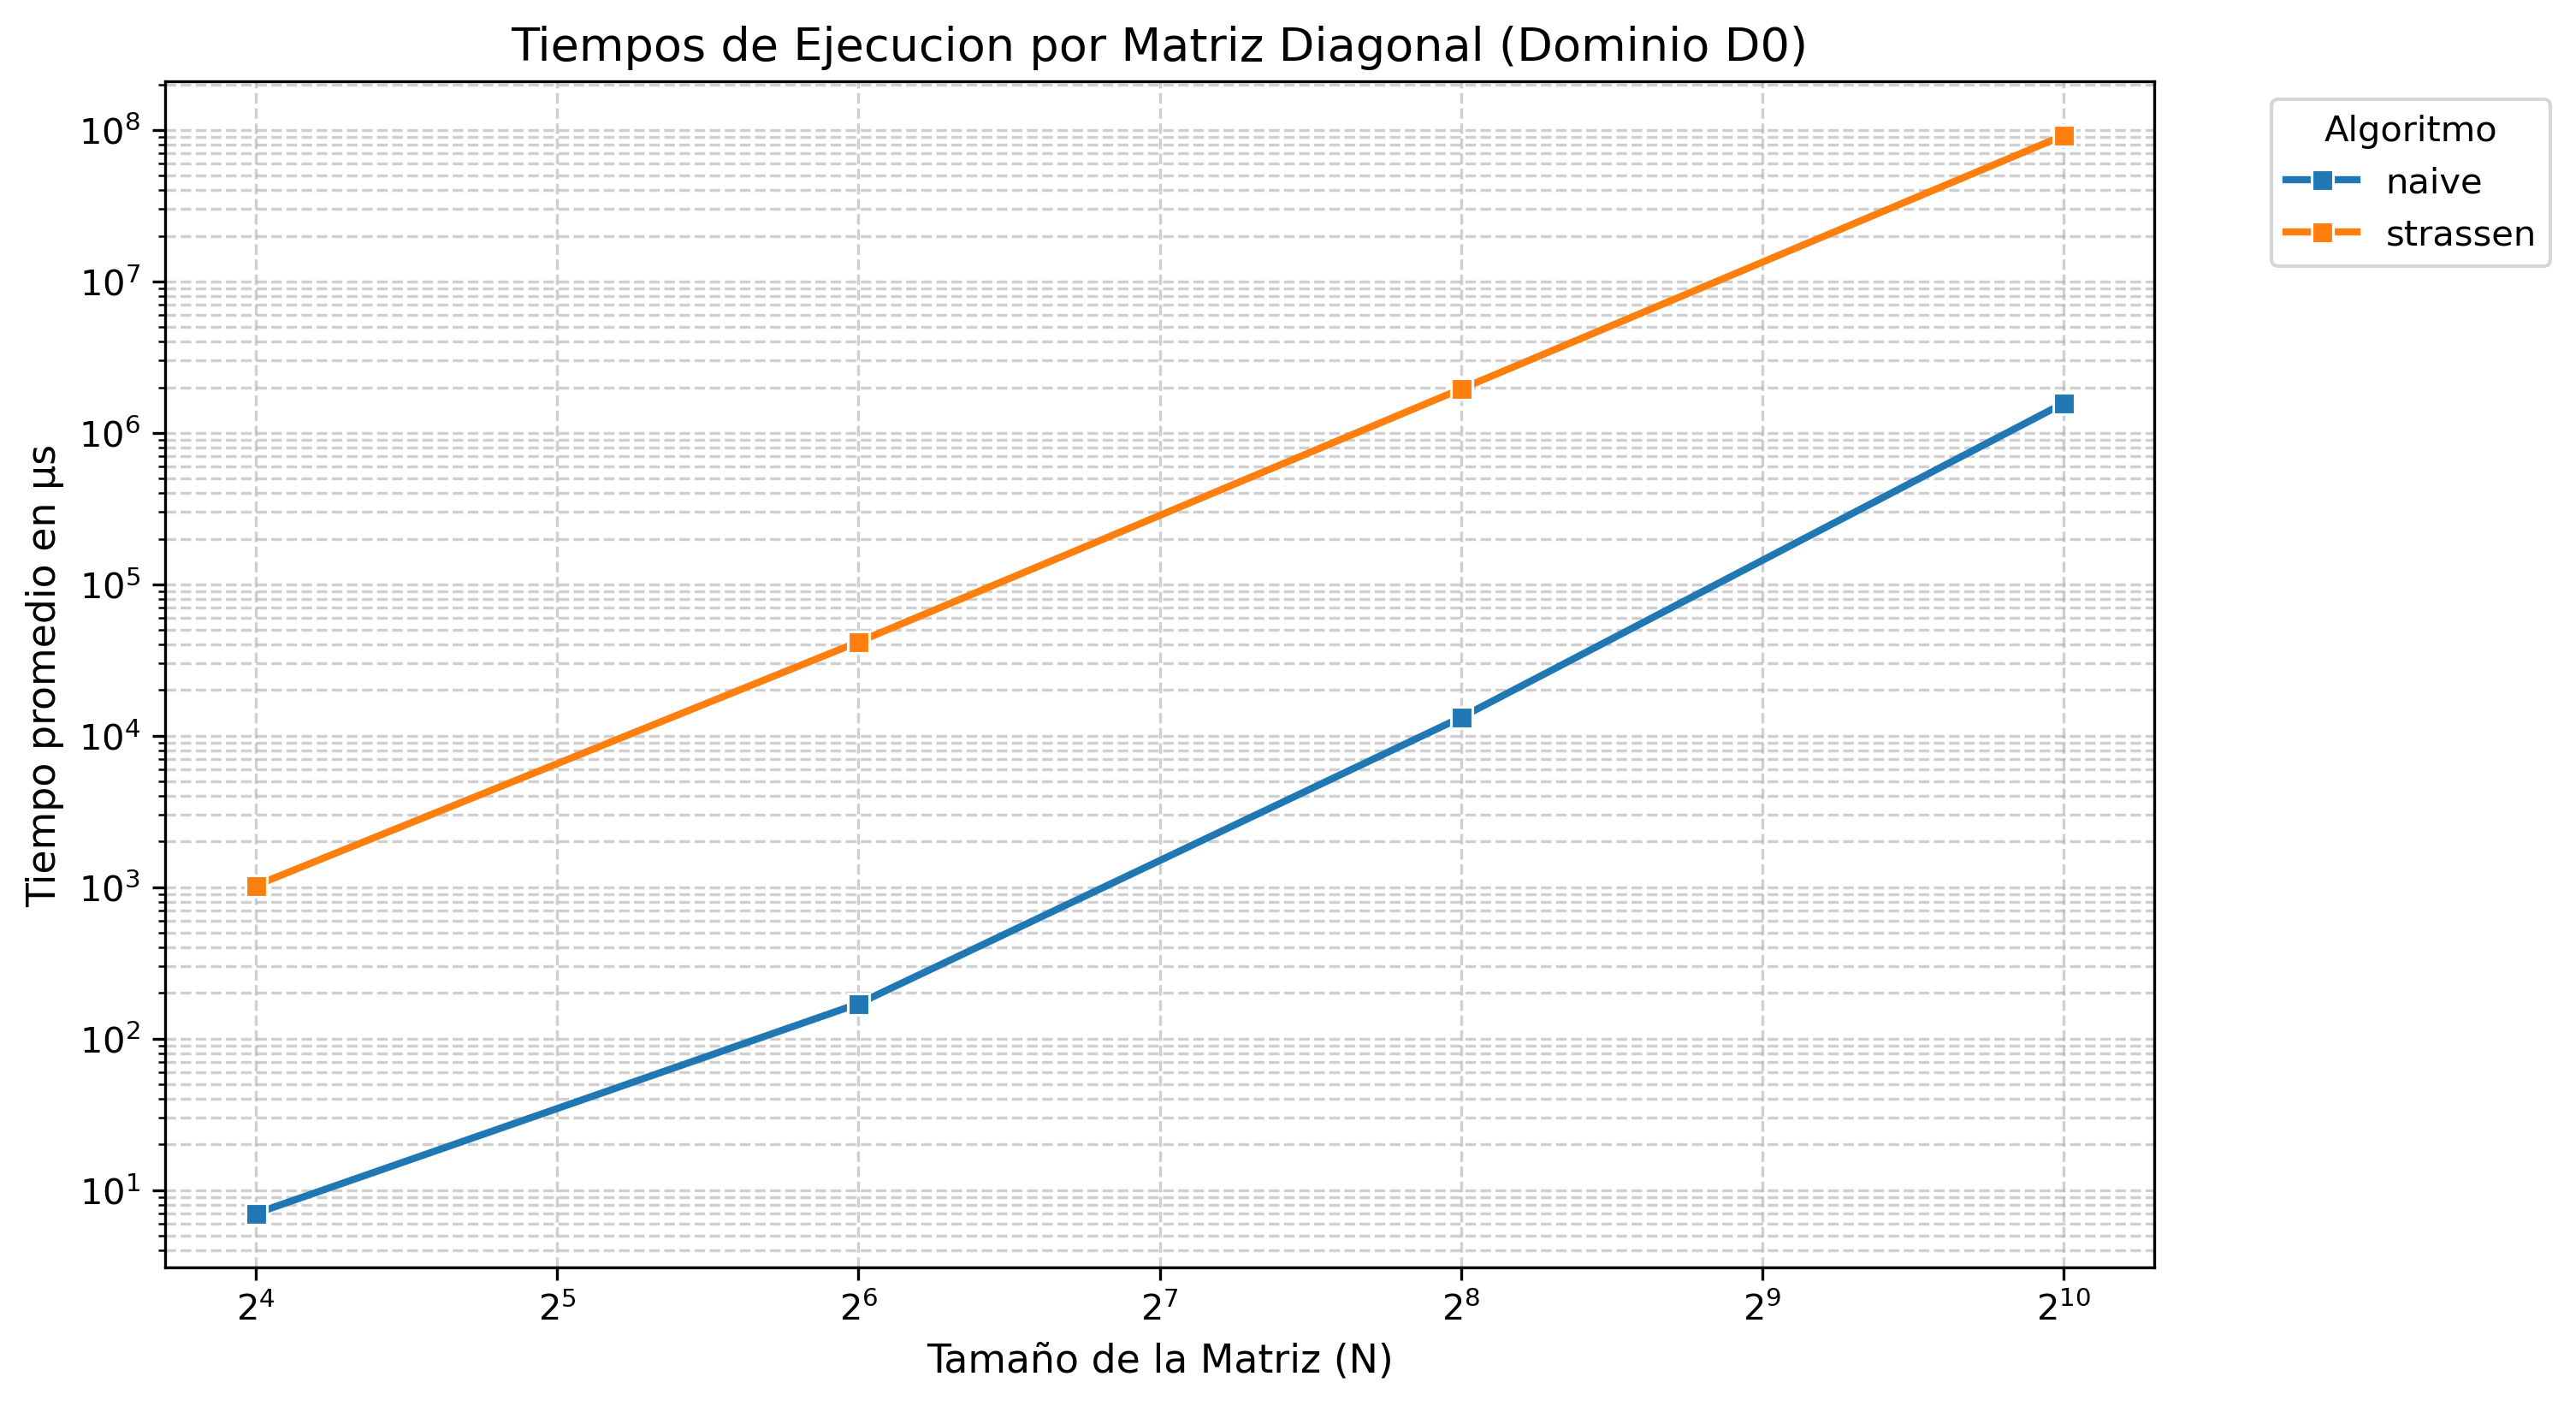
\includegraphics[width=0.85\textwidth]{../code/matrix_multiplication/data/plots/plot_diagonal_D0.png}
    \caption{Matriz Diagonal (D0)}
\end{figure}